\section{Appendix} \label{sec: Appendix}
The appendix contains code listening and other large information parts that contain partial or complete relevance to the reports topic. 

\subsection{Lesson Learned} \label{subsec: Lesson Learned}
\subsubsection{Vivado Language Templates} \label{subsubsec: Vivado Language Templates}
Figure \ref{fig: Vivado_LanguageTemplates} shows a handy tool build into Vivado software package that is called Language Templates and it seems to contain most of the verilog syntax.
\begin{figure}[htbp]
	\centering
	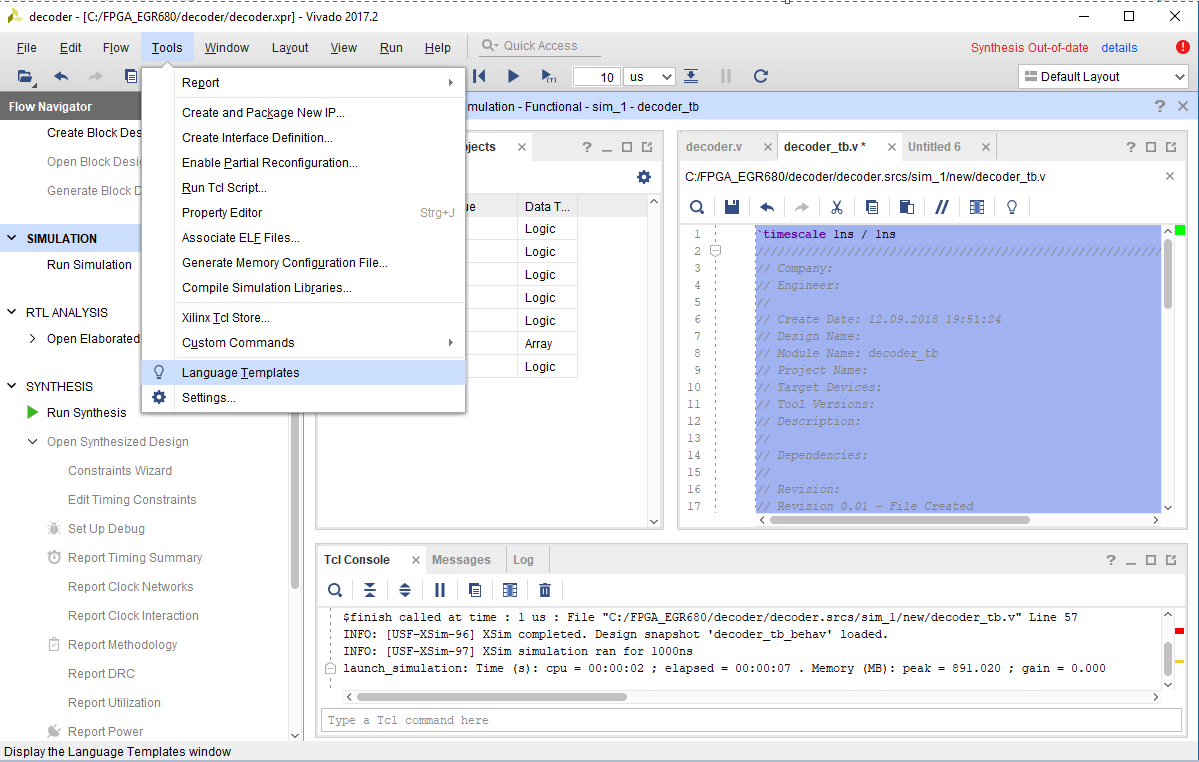
\includegraphics[width=0.6\textwidth]{01_images/Vivado_LanguageTemplates.png}
	\caption{Vivado Language Templates.}
	\label{fig: Vivado_LanguageTemplates}
\end{figure}
\subsubsection{Clock divider not working} \label{subsubsec: Clock divider not working}
Listening \ref{lst: clock divider issue} shows a code snipe out of the clock divider that caused a lot of trouble by preventing the clock divider preventing dividing the clock. It seems that the last statement $clk_out <= clk_out;$ overwrote the statement 
$clk_out <= ~clk_out;$ which results either in an unknown state or an zero on the divided clock instead of the desired toggling clock behavior. 
\begin{lstlisting}[language=verilog,caption={Clock divider issue.},label=lst: clock divider issue]
else
begin

clk_temp <= clk_temp + 1;
if (clk_temp >= 500000) 
//if (clk_temp >= 2) // Used for testbench
begin
clk_out <= ~clk_out; // no clue why this line does not toggle the clk_out
//   if (clk_out == 0) 
//   begin
//   clk_out=1;
//   end 
//   else
//   begin
//   clk_out=0;
//   end
clk_temp <= 0;
end
end // else rst
//clk_out <= clk_out; // could this lane of HDL be causong the problem of the not working clk divider? Yes, it is!!!

\end{lstlisting}
